\chapter{Related work}
\label{cha:related}

In this chapter will deepen on the SAT-to-Ising reduction problem, which has been proved to be useful when trying to exploit properties of quantum computing to reduce the computation time to solve SAT problems. We will discuss a preliminary algorithm that have been studied at University of Trento, distinguishing the procedure adopted to encode simple formulas from complex Boolean instances.

\section{SAT-to-Ising}
\label{sec:SATtoQUBO}

As already stated in the previous paragraphs, SAT main issue is the exponential growth of complexity, stopping computer scientists in investigating hard tasks involving a small number of variables. Quantum computing, on the other hand, exploit specific phenomena such as tunneling to search the minimum of an Ising problem, optimizing computational time. If we would be able to encode SAT/MaxSAT problem into an Ising Hamiltonian problem, we could exploit quantum calculus properties to verify satisfiability of out original problems, drastically reducing computational time. The task described is known as \textbf{SAT-to-QUBO}. \\
Computer scientists use Quantum Annealers as black-box algorithms which are fed to QUBO problems, whose formulation is similar but not identical to an Ising problem:

\begin{equation}
    H(\textbf{\underline{z}}) =\theta + \sum_{i \in V} h_iz_i + \sum_{\langle i,j\rangle \in E} J_{ij} z_iz_j
\end{equation}

As we can see qubits, biases and couplings are present in our formulation; in addition to them we consider the parameter $\theta_0$, which is called offset and falls into the range $(+\infty, -\infty)$. \\
Given a SAT problem, we are interested in finding a variable placement \textbf{x} $\rightarrow$ \textbf{z} on the quantum annealer qubits and the values of offset, biases and couplings so that:

\begin{equation}
    P_F(\underline{\textbf{x}} | \underline{\theta}) = 
    \left\{
        \begin{array}{lr}
            = 0, & if \textbf{ \underline{x}} \models F \\
            \geq g_{min}, & if \textbf{ \underline{x}} \models T
        \end{array}
    \right\}
\end{equation}

The gap $g_{min}$ is essential to manage sensitivity of the quantum annealer: the optimization will be affected by noise generated by the non-zero Kelvin temperature and , so it will be rarely the case that not satisfying assignment will get 0 as final score. Setting the gap (and trying to find the highest gap possible satisfying the problem) will help us in discriminating acceptable assignments and not acceptable ones.
For instance, a formula we can easily encode into an Ising Hamiltonian function is $\varphi = x_1 \iff x_2$. A simple penalty function would be $P_F(\underline{\textbf{x}} | \underline{\theta}) = 1 - x_1x_2$, whose gap for satisfying assignment is 2. \\
The current formulation of our problem presents some issues:

\begin{itemize}
    \item Chimera tile architecture is quite limited: the absence of clique and the sparsity of the matrix reduce the number of problem we can represent.
    \item The problem is actually overconstrained: you need to search your solution checking O($2^{|\textbf{\underline{x}}|}$) models/countermodels. You have also to deal with the degrees of freedom of its formulation caused by biases and couplings.
\end{itemize}

To overcome this difficulties, we can add a non-fixed numbers of ancillary variables to provide the missing links. The problem will slightly change into the task:

\begin{equation}
    min_{[\textbf{\underline{a}} \in \{-1,1\}^k]} P_F(\underline{\textbf{x}},\underline{\textbf{a}} | \underline{\theta}) = 
    \left\{
        \begin{array}{lr}
            = 0, & if \textbf{ \underline{x}} \models F \\
            \geq g_{min}, & if \textbf{ \underline{x}} \models T
        \end{array}
    \right\}
\end{equation}

The more ancillary variables we add to our formulation, the more complex the resulting task will be, so we will always try to limit their use only when necessary. Ancillary variable are essential for basic encoding formulas: an example could be $\varphi = x_3 \iff (x_1 \vee x_2)$. If the Quantum Annealer admitted cliques the encoding would be trivial; since this is not the case, an ancilla is added to obtain a valid penalty function:

\begin{equation}
    P_F(\underline{\textbf{x}},\underline{\textbf{a}} | \underline{\theta}) = \frac{5}{2} - \frac{1}{2} x_1 - \frac{1}{2} x_2 + x_3 + \frac{1}{2} x_1x_2 - x_1x_3 - x_2a -x_3a
\end{equation}

Figure 1.3 shows the positioning of the obtained Ising Hamiltonian functions into a Chimera tile.
\begin{figure}[t]
	\begin{center}
	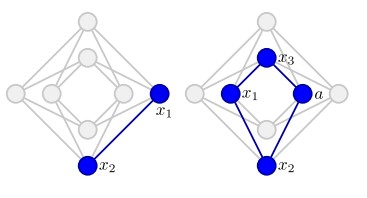
\includegraphics{images/Ising1+2.png}
	\caption{On the left, a valid positioning of qubits into a Chimera tile for the formula $\varphi = x_1 \iff x_2$. On the right, a valid positioning for the formula $\varphi ' = x_3 \iff (x_1 \vee x_2)$. Both architectures are inspired by the penalty functions discussed in this paragraph.}
	\end{center}
\end{figure}

\section{Issues in Encoding for Quantum Annealers}

Converting a Boolean circuit into a QUBO formulation would apparently seem an easy task to achieve: actually the nature and the architecture of the annealers drastically reduce the number of SAT problems we can embed. The main issues causing the inefficiency are:

\begin{itemize}
    \item \textbf{The number of qubits is not unlimited}: even though the recent architectures provides more than 2000 qubits, they are usually not enough to encode the majority of circuits.
    This is due by the nature of the two encoding: the number of qubits representing the input width and the circuit size are two different metrics for complexity, where the former is definitively bigger than the latter. 
    \item \textbf{The number of couplings is not unlimited}: as already mentioned in paragraph, each architecture can be interconnected to a limited number of other qubits. Consequently, the encoding process has to take into account this upper limit and, if more connections are required, map a Boolean variable into multiple qubits.
    \item \textbf{Noise impacts the system performance}: the ideal condition of a quantum annealer would require a temperature of 0 K and to be heavily shielded by electro-magnetic rays, preserving the properties of the superconductor rings. In reality these conditions are never met and D-Wave system are subject to performance degradation.
\end{itemize}

Because of the problems described above, advanced algorithms have been studied and tested in order to reduce the amount of qubits required during the reduction of the SAT circuit.


\section{Encoding complex Boolean formulas}

Determine an efficient encoding is decisive, given the limited of number of qubits of Chimera. Penalty functions have some properties we can exploit to iteratively build complex formula from easier ones. The first property is \textbf{NPN-Equivalence}: given a boolean formula $F(\textbf{\underline{x}})$ with its associated penalty function $P_F(\underline{\textbf{x}},\underline{\textbf{a}} | \underline{\theta})$ and a new Boolean function $F^*(\textbf{\underline{x}})$ identical to the previous one but a single variable at a generic index $i$ (so that it appears with inverse cardinality in the new formulation), we can recycle $P_F(\underline{\textbf{x}},\underline{\textbf{a}} | \underline{\theta})$ to obtain the penalty function for the new problem. In particular, $P_{F^*}(\underline{\textbf{x}},\underline{\textbf{a}} | \underline{\theta}) = P_F(\underline{\textbf{x}},\underline{\textbf{a}} | \underline{\theta}^*)$ where $\theta^*$ is a new vector of biases and couplings so that for each $z,z'\in \textbf{\underline{x}},\textbf{\underline{a}}$: \\ \\ \\

\begin{equation}
    \theta_z^* = 
    \left\{
        \begin{array}{lr}
            -\theta_z, & \textit{if }z = x_i \\
            \theta_z, & otherwise
        \end{array}
    \right\}
\end{equation}

\begin{equation}
    \theta_{zz'} = 
    \left\{
        \begin{array}{lr}
            -\theta_{zz'}, & \textit{if }z = x_i \vee z' = x_i\\
            \theta_{zz'}, & otherwise
        \end{array}
    \right\}
\end{equation}


So once we extract the penalty function for a Boolean Formula, its variants can be easily computed switching signs of biases and coupling. For instance, if we had the Boolean formula $\varphi = x_1 \iff -x_2$, we could easily invert signs of couplings and biases associated with $x_2$, trivially obtaining $P_F(\underline{\textbf{x}} | \underline{\theta}) = 1 + x_1x_2$. \\
The second property fundamental to simplify the task of retrieving penalty functions is the \textbf{AND-decomposition}. Given a Boolean function that can be rewritten as a combination of simpler functions so that $F(x) = \land_k F_k(\underline{x}^k)$, where each $F_k(x)$ is associated to a penalty function $P_{F_k}(\underline{x^k},\underline{a^k}|\underline{\theta^k})$ with minimum gap $g^k_{min}$, $\underline{x} = \cup_k \underline{x^k}$ and $\underline{a} = \cup_k \underline{a^k}$, then we can define a penalty function for the original formula in the following way:

\begin{equation*}
    P_{F}(\underline{x},\underline{a}|\underline{\theta}) = \sum_k P_{F_k}(\underline{x^k},\underline{a^k}|\underline{\theta^k}) \; \textrm{        with        } g_{min} = \min_k(g^k_{min})
\end{equation*}
\begin{equation}
    \theta_i = \sum_k \theta^k_i
\end{equation}
\begin{equation*}
    \theta_{ij} = \sum_k \theta^k_{ij}
\end{equation*}

Equation 2.8 works in the case each bias and coupler value satisfies its range. The subformulas making up the decomposition could share some common variables and, in some cases, this could lead to the attainment of out-of-range biases and couplers. This issue can be easily fixed: we can scale up or down the impact of each penalty function adding a weight $w_k$ greater than 0. This addition slightly modifies equation 2.8, determining the general formulation:

\begin{equation*}
    P_{F}(\underline{x},\underline{a}|\underline{\theta}) = \sum_k P_{F_k}(\underline{x^k},\underline{a^k}|\underline{\theta^k})*w_k \; \textrm{        with        } g_{min} = \min_k(g^k_{min})*w_k
\end{equation*}
\begin{equation}
    \theta_i = \sum_k \theta^k_i*w_k
\end{equation}
\begin{equation*}
    \theta_{ij} = \sum_k \theta^k_{ij}*w_k
\end{equation*}

Adding these weights weakens the minimum gap, so it is not used in practice. An alternative to equation 2.9 relies on the renaming of the shared variable, so that each $\underline{x}^k$ is disjoint with respect to the others. To achieve this goal, when two conjuncts $F_k, F'_k$ share a Boolean variable $x_i$ we rename the second occurrence with a fresh variable $x'_i$ and conjoin the two variable using the simple formula $(x_i \iff x'_i)$. Now we can re-define the original formula and its associated penalty function as:

\begin{equation*}
    F^*(\underline{x}^*) = \bigwedge_k F_k(\underline{x}^{k*}) \land \bigwedge_{\{ x_i \textrm{  shared}\}} (x_i \iff x'_i) 
\end{equation*}
\begin{equation}
    P_{F^*}(\underline{x}^*,\underline{a}|\underline{\theta}) = \sum_k P_{F_k}(\underline{x^k},\underline{a^k}|\underline{\theta^k}) + \sum_{\{ x_i \textrm{  shared}\}} (1 - x_ix'_i)
\end{equation}
\begin{equation*}
    g_{min} = min_k(g^k_{min},2)
\end{equation*}

Given the nature of the penalty functions for $(x_i \iff x'_i)$, whose gap is 2, we ensure no issue can emerge and no parameter range error can be observed.
Combining the two properties above we can define the procedure to apply to retrieve penalty functions decomposing Boolean formulas into smaller chunks, easier to convert:

\begin{itemize}
    \item First we Tseitin-style decompose $F(x)$ into an equi-satisfiable formula so that:
    
    \begin{equation}
        F*(\underline{x},\underline{y}) = \bigwedge^{m-1}_{i=1} 
        (y_i \iff F(\underline{x}^i,\underline{y}^i)) \wedge F_m(\underline{x}^m,\underline{y}^m)
    \end{equation}
    
    \item When two conjuncts $F_1$ and $F_2$ share one variable $y_j$, rename the second with a fresh new variable $y_i'$, conjoining $(y_i' \iff y_j)$.
    \item Compute the penalty function for each conjunct separately.
    \item Sum the penalty functions obtained in the previous step to obtain a single function. 
\end{itemize}

From the algorithm described above, we can define a universal approach to deal with larger Boolean functions, avoiding the application of the SMT formulation which results too much time and resource demanding. \\
Before starting the encoding, we compute in advance a collection of valid encoding for simple SAT formulas so that they can be mapped using a low number of qubits (in particular when using the Chimera architecture we aim to encode the formula using a single tile). The original SAT formula we want to encode is pre-processed, in order to reduce its size or complexity in terms of its graphical
representation. As an example, a good pre-processing approach is using the and-inverted-graph representation, which transform a formula in a combination of AND and NOT functions. Using the simplified structure and the previously computed library we then define a mapping between Boolean variables and the annealer's qubits. This phase represents the most complex and resource-demanding procedure of the algorithm. The fundamental steps of this procedure are:

\begin{figure}[t]
	\begin{center}
	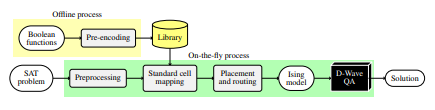
\includegraphics[width=\textwidth]{images/LargeBool.PNG}
	\caption{A graphical representation of the encoding process for larger Boolean functions.}
	\end{center}
\end{figure}

\begin{itemize}
    \item Use the library of pre-computed penalty functions to map each function part of the decomposed and simplified SAT formula into a valid QUBO encoding. This phase is known as standard cell mapping.
    \item Now it is necessary to embed the entire formula onto the QA hardware. To achieve this task, we first assign a disjoint subgraph of the QA hardware graph to each penalty function chosen in the previous step.
    \item Lastly we need to ensure that qubits representing the same variable are chained so that they can assume the same value when given as input to the annealer: we can accomplish it using penalty functions in the form $1 - x_1x_2$, where $x_1$ and $x_2$ are qubits representing the same variable. This step is a direct consequence to formula 2.8.
\end{itemize}

The algorithm is heavily discussed in \cite{varotti} and more details are provided about the choice of and the heuristic adopted to obtain a more stable encoding, but for the sake of brevity we will not discuss it further. Figure 2.4 summarizes the entire process.

\pagebreak